\section{Compacité}
\begin{definition}
   Soit $F \subset E$. Un recouvrement ouvert de $F$ est une collection  $(U_i)_{i \in I}$ où $U_i$ sont des ouverts et $F \subset \cup_{i \in I} U_i$ ("les $U_i$ recouvrent  $F$")
\end{definition}
\begin{eg}
\begin{figure}[H]
    \centering
    \incfig{recouvrement-ouvert}
    \caption{recouvrement-ouvert}
    \label{fig:recouvrement-ouvert}
\end{figure}
\begin{itemize}
    \item $U_x = B(x, \frac{1}{2})$
    \item $\bigcup_{x \in F} U_x$ contient $F$
    \item  $(U_x)_{x \in F}$ recouvrement ouvert de $F$
\end{itemize}
\end{eg}

\begin{definition}
    $K \subset E$ est compact si de tout recouvrement ouvert $(U_i)_{i \in I}$ de $F$ on peut extraire un sous-recouvrement fini: je peux choisir  $i_1, \ldots, i_n \in I$ tels que 
    \[
    F \subset U_{i_1} \cup U_{i_2} \cup \ldots \cup U_{i_n}
    \] 
\end{definition}
\begin{property}
   Un ensemble fini est compact. 
   \[
       F = \{a_1, \ldots, a_p\} \quad a_j \in E
   \] 
   $(U_i)_{i \in I}$ recouvre $F$.
   Je choisit  $a_j$ (point de $F$), il existe un $i \in I$ noté  $i(j)$ tel que 
    \[
   a_j \in U_{i(j)} \quad F \subset U_{i(1)} \cup \ldots \cup U_{i(p)}
   \] 
\end{property}
\begin{theorem}
    Caractérisation à l'aide de suites. \par
    $K \subset E$ est compact ssi toute suite d'éléments de $K$ admet une sous-suite qui converge vers un élément de  $K$.
\end{theorem}
\begin{eg}
    \begin{figure}[H]
        \centering
        \incfig{compactness-with-sequences}
        \caption{compactness-with-sequences}
        \label{fig:compactness-with-sequences}
    \end{figure}
    \begin{itemize}
        \item $E = \R^2$
        \item $F = B(x_0, r)$ pas compact
        \item $x_n \in F$,  $x_n \to x$, $x \not\in F$
        \item si $y_n = x_{\phi(n)}$, $y_n \to x$ mais $x \not\in F$
    \end{itemize}
\end{eg}
\begin{eg}
    
\begin{figure}[H]
    \centering
    \incfig{suite-sans-sous-suite-convergente}
    \caption{suite-sans-sous-suite-convergente}
    \label{fig:suite-sans-sous-suite-convergente}
\end{figure}
\[
    F = \{(x, y): x \ge 0, -\frac{1}{x} \le y \le \frac{1}{x} \}
\] 
$u_n = (n, 0)$  $(u_n)$ suite dans  $F$ sans sous-suite convergente.
\end{eg}

\begin{prop}
    \begin{enumerate}
        \item $K$ compact $\implies$ $K$ fermé et borné. (réciproque est fausse en général!)
        \item Si $K$ compact et $F$ fermé, alors  $K \cap F$ est compact.
        \item Si $K$ compact, toute suite de Cauchy dans  $K$ converge dans  $K$
    \end{enumerate}
\end{prop}

\begin{preuve}
   \begin{enumerate}
       \item Soit $K$ compact.  $K$ fermé si  $(u_n)$ suite dans  $K$ qui converge vers  $u$, alors  $u \in K$.
           \par
           \underline{clair:}  $(u_n)$ a une suite-suite  $v_n = u_{\phi(n)}$ avec $v_n \to v \in K$, $u_n \to u$, donc $v_n \to u$ $\implies$ $u = v$  $\implies$ $u \in K$
           \par
           $K$ \underline{est borné}:
           \par
              Soit $U_x = \bigcup_{x \in K} B(x, 1)$ un recouvrement ouvert de $K$. Or  $K$ est compact, donc il existent  $x_1, \ldots, x_n \in K$, tels que $K \subset \bigcup_{i = 1, \ldots, n} B(x_i, 1) $, donc $K$ est borné.
        \item $K$ compact et $F$ fermé. $(u_n)$ une suite dans $K \cap F$. $u_n \in K$. $ \exists$ sous-suite $v_n = u_{\phi(n)}$ avec $v_n \to x \in K$. $v_n \in F, v_n \to x$, $F$ fermé donc $x \in F$, $x \in K \cap F$.
        \item Sout $(u_n)$ suite de Cauchy dans $K$. $(u_n)$ a une sous-suite $v_n = u_ { \phi(n)}$ qui converge vers $x \in K$. $u_n \to x \in K$
   \end{enumerate} 
\end{preuve}

\subsection{Compacité dans $\R^n$ avec la distance usuelle}
\begin{theorem}
    (Borel-Lebesgue)
    \par
    dans $\R^n$ avec la distance usuelle $K$ est compact ssi  $K$ est fermé et borné
\end{theorem}

\begin{prop}\label{prop:boules-fermes-sont-compactes}
   Les boules fermées $B_f(x_0, r)$ sont compactes dans $\R^n$. 
\end{prop}
\begin{itemize}
    \item Implique le théorème: Soit $K$ fermé et borné.  $K$ borné, donc  $K \subset B_f(0, r)$ avec $r$ grand, donc  $K = K \cap B_f(0, r)$. Donc  $K$ compact.
\end{itemize}
\begin{preuve} de la prop. \ref{prop:boules-fermes-sont-compactes}
   \begin{enumerate}
       \item $n = 1$.  À montrer: $[a, b]$ est compact.
           \par
           Soit  $(U_i)_{i \in I}$ un recouvrement ouvert de $[a, b]$. Soit  $F$: les  $x \in [a, b]$ tels que  $[a, x]$ est récouvert par un nombre fini de  $U_i$.
           \par
           \underline{But:} montrer que  $b \in F$! (si $x \in F$, et  $x' \le x$ $x' \in F$)
            \begin{enumerate}
                \item $F \neq \O$: $a \in F$  $[a, a] = \{ a \}$
                \item  $c = sup(F)$. \underline{On montre que $c = b$} \par
                    Supposons que $c < b$.
                     \begin{itemize}
                        \item $c$ appartient à un des  $U_i$ noté  $U_{i_0}$
                        \item $U_{i_0}$ est ouvert, $c \in U_{i_0}$ donc $\exists \delta_0 > 0$ tel que $]c - \delta_0, c + \delta_0[ \subset U_{i_0}$
                        \item $c = sup(F)$:  $\forall \delta > 0, \, \exists x_{\delta} \in F$ avec $c - \delta < x_{\delta} \le c$
                            \[
                            \delta = \delta_{0,2} \quad \exists x_{\delta_0} \in F, c - \delta_{0,2} < x_{\delta_0}
                            \] 
                            $[a, x_{\delta_0}]$ reouvert par $U_{i_1} \cup \ldots \cup U_{i_n}$ et $]c - \delta_0, c + \delta_0[ \subset U_{i_0}$ donc $[a, c + \delta_{0,2}]$ est reouvert par $U_{i_0} \cup U_{i_1} \cup \ldots \cup U_{i_n}$, donc $c + \delta_{0, 2} \in F$ contredit que $c = sup(F)$. Donc  $c = b$.
                            \par
                            $F$ c'est  $[a, b[$ ou $[a, b]$.  $b \in F$  $\exists U_{i_1}, \ldots, U_{i_n}$ tq $[a, b] \subset U_{i_1} \cup \ldots \cup U_{i_n}$, $[a, b]$ compact.
                    \end{itemize}
            \end{enumerate}
   \end{enumerate}
\end{preuve}

\section{Limites et continuité}
\subsection{Limites}
Je prends $(E_1, d_1), (E_2, d_2)$ deux espaces métriques et $F: E_1 \to E_2$. $x_0 \in E_1, l \in E_2$.
\begin{definition}.
    \begin{enumerate}
        \item Limite:
            \[
            \lim_{x \to x_0} F(x) = l
            \] 
            si $\forall \epsilon > 0, \exists \delta > 0$ tq si $d_1(x_0, x) < \delta$ alors $d_2(l, F(x)) < \epsilon$
        \item $F$ continue en  $x_0$ si $\lim_{x \to x_0} F(x) = F(x_0)$
        \item $F$ est continue (sur $E$) si elle est continue en tout $x_0$ de $E$
\end{enumerate}
\end{definition}
\begin{prop}
   Les propriétés suivantes sont équivalentes: 
   \begin{enumerate}
       \item $F: (E_1, d_1) \to  (E_2, d_2)$ est continue.
       \item $\forall U_2 \subset  E_2$ ouvert, $F^{-1}(U_2)$ est ouvert dans $E_1$.
       \item $\forall F_2 \subset E_2$ fermé, $F^{-1}(F_2) \subset E_1$ est fermé.
        \item $\forall (x_n)$ suite dans $E_1$ avec $\lim_{n \to \infty} x_n = x$ on a:
            \[
            \lim_{n \to \infty} F(x_n) = F(x)
            \] 
   \end{enumerate}
\end{prop}
\begin{figure}[H]
    \centering
    \incfig{continuite-topologique}
    \caption{continuite-topologique}
    \label{fig:continuite-topologique}
\end{figure}
\begin{eg}
   \[
       U = \{(x, y) \in \R^2: x \sin(y) - e^x > 1\}
   \]  
   \begin{align*}
       F: \R^2 &\longrightarrow \R \\
       (x, y) &\longmapsto F((x, y)) = x \sin(y) - e^x
   \end{align*}
   évidemment continue.
   \[
       U = F^{-1}(\underbrace{]1, +\infty[}_{\text{ouvert de } \R})
   \] 
\end{eg}
\begin{preuve}
   $1 \implies 2 \implies 3 \implies 4 \implies 1$ 
   \begin{itemize}
       \item[$1 \implies 2$:] Hyp: $F$ continue et  $U_2 \subset E_2$ est ouvert.
           \par
           Conclusion: $U_1 = F^{-1}(U_2)$ est ouvert?
           \par
           Je fixe $x_0 \in U_1$ ($F(x_0) \in U_2$).
           \begin{enumerate}
               \item $U_2$ ouvert $\implies$ $\exists \epsilon_0 > 0$ tq $B_2(F(x_0), \epsilon_0) \subset U_2$
               \item $F$ continue en  $x_0$: 
                   \[
                   \forall \epsilon > 0, \, \exists \delta > 0 \text{ tq } d_1(x_0, x) < \delta \implies d_2(F(x_0), F(x)) < \epsilon
                   \] 
                   \[
                   x \in B_1(x_0, \delta) \implies F(x) \in B_2(F(x_0), \epsilon)
                   \] 
                   $\delta_0 = $ le  $\delta$ qui marche pour  $\epsilon_0$
                    \[
                   x \in B_1(x_0, \delta_0) \implies F(x) \in B_2(F(x_0), \epsilon_0)
                   \] 
                   Donc $B_1(x_0, \delta_0) \subset F^{-1}(U_2)$. Donc $F^{-1}(U_2)$ ouvert.
           \end{enumerate}
       \item[$2 \implies 3$:]: $F^{-1}(U_2)^{c} = F^{-1}(U_2^c)$
   \end{itemize}
\end{preuve}

\begin{eg} résultat de cette proposition.
    Prenons la fonction: $f(x) = x^2$.  $f^{-1}(]4, 9[) = \{x \in \R \mid 4 < x^2 < 9\} = ]-3, -2[ \cup ]2, 3[$. Autrement dire, la continuité de $f$ (évident) donne que  $U = ]4, 9[$ ouvert, alors $f^{-1}(U)$ aussi ouvert.
    \begin{figure}[H]
        \centering
        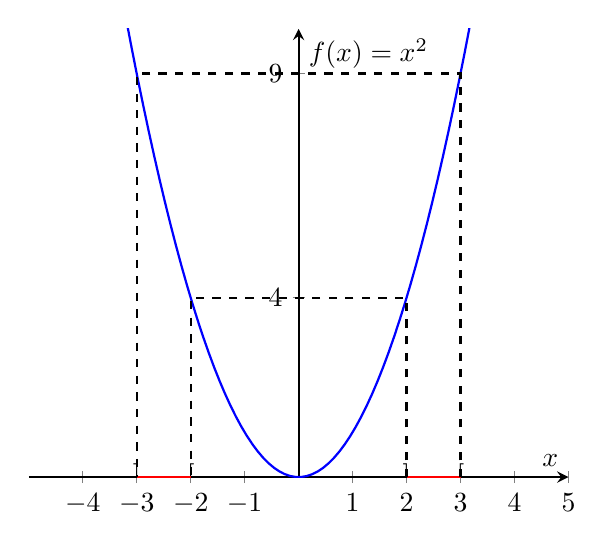
\begin{tikzpicture}
            \begin{axis}[
                axis lines = middle,
                xlabel = $x$,
                ylabel = {$f(x) = x^2$},
                xmin=-5, xmax=5,
                ymin=0, ymax=10,
                samples=100,
                domain=-5:5,
                xtick={-4,-3,-2,-1,0,1,2,3,4,5},  % Custom x-axis numbers
                ytick={0,4,9},   % Custom y-axis numbers
                thick
                ]
                \addplot[blue, thick] {x^2};
                \coordinate (a) at (2, 0);
                \node (_) at (a){$]$};
                \coordinate (b) at (-2, 0);
                \node (_) at (b){$[$};
                \coordinate (c) at (3, 0);
                \node (_) at (c){$[$};
                \coordinate (d) at (-3, 0);
                \node (_) at (d){$]$};

                \coordinate (fa) at (2, 4);
                \coordinate (fb) at (-2, 4);
                \coordinate (fc) at (3, 9);
                \coordinate (fd) at (-3, 9);
                \draw[color=red] (a) -- (c);
                \draw[color=red] (b) -- (d);

                \draw[dashed] (a) -- (fa) -- (fb) -- (b);
                \draw[dashed] (c) -- (fc) -- (fd) -- (d);
            \end{axis}
        \end{tikzpicture} 
        \caption{Exemple en $f(x) = x^2$}
    \end{figure}
\end{eg}
